
\section{Motion with naive MLA}
\label{sec:naive_mla}
We have so far only focused on perfect MLA, so it would be interesting to see if real MLA induces artifacts. There exist several MLA approaches (\cite{prb_approaches}), but we choose to experiment with a naive approach to MLA. For each transmit beam, three receive beams with different focus points are created by time-delaying the recorded data. With this naive approach, the magnitude of the receive beams is not corrected to compensate for the difference in the energy sent towards their focus point.

In this example, the receive beams are built such that they are uniformly distributed along the image azimuth. If $d_B$ is the distance between two transmit beam, the receive beams are built with focus points shifted $\{-d_B/3, 0, d_B/3\}~$mm from those of the transmit beams.
The experiment of Figure \ref{fig:loss_vs_beams}, where the beamformers' maximum scalloping loss is estimated for different beam densities, is repeated in Figure \ref{fig:loss_vs_beams_mla} with varying transmit beam densities $b_{tr}$ and $b_{re} = 3 \cdot b_{tr}$.
\begin{figure}[ht]
    \centering
    \begin{subfigure}[t]{\linewidth}
        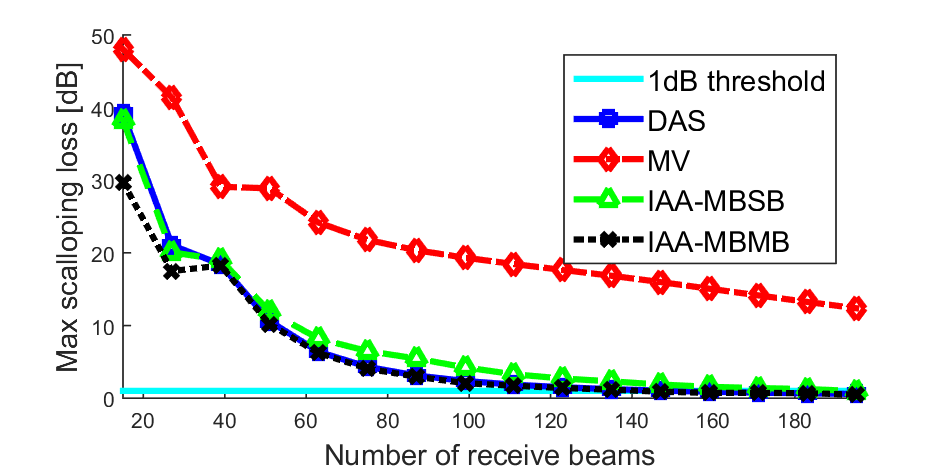
\includegraphics[width=\linewidth]{./images/results/4/loss_vs_beams_mla.png}
        \caption{Maximum scalloping loss of DAS, MV, IAA-MBSB and IAA-MBMB beamformers for $b_{re} \in [15, 195]$.}
    \end{subfigure}
    \quad
    \begin{subfigure}[t]{\linewidth}
        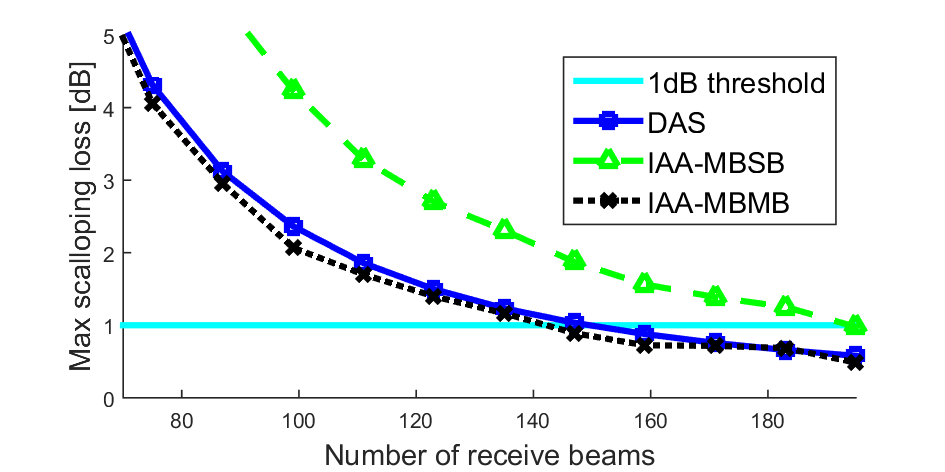
\includegraphics[width=\linewidth]{./images/results/4/loss_vs_beams_mla_zoom.png}
        \caption{Maximum scalloping loss of DAS, IAA-MBSB and IAA-MBMB beamformers for $b_{re} \in [75, 195]$.}
    \end{subfigure}
	\caption[Maximum scalloping loss of single scatterer point at $40~mm$ radius in noiseless medium with naive MLA.]{Maximum scalloping loss of single scatterer point at $40~mm$ radius in noiseless medium with naive MLA. All beamformers use MLA with $b_{re} = 3 \cdot b_{tr}$. The maximum scalloping loss values of all beamformers for $b_{re} \in [15, 195]$ are dispalyed in (a). For enhanced visibility, a focus on the DAS, IAA-MBSB and IAA-MBMB values for $b_{re} \in [75, 195]$ is provided in (b).}
	\label{fig:loss_vs_beams_mla}
\end{figure}

Since no beam correction is done, the beamformers are generally experiencing higher scalloping loss than with perfect MLA. However naive MLA converges towards perfect MLA for high beam densities, since little correction is then required.
For that reason, the MV and IAA-MBSB require roughly the same $b_{re}$ threshold to become shift-invariant with SLA, or perfect MLA, and naive MLA, whereas the $b_{re}$ threshold for DAS is significantly higher with naive MLA ($b_{re} = 145$) than with SLA ($b_{re} = 65$).
We can notice though that the IAA-MBMB beamformer impressively yields a lower $b_{re}$ threshold with naive MLA than with SLA.
As explained in Section \ref{sec:res_frames_motion}, we can reasonably expect the multibeam beamformers to roughly correct for scalloping loss by combining overlapping beams in directions where scalloping loss occurs.
However, we did not expect the IAA-MBMB to require fewer receive beams when using MLA without scalloping loss correction than when using SLA.
In order to have a closer look at this issue, we can take a look at the actual maximum and minimum gains of the imaged scatterer point instead of their difference, which is the maximum scalloping loss.
This gain decomposition is done both for the SLA (Figure \ref{fig:loss_vs_beams}) and MLA (Figure \ref{fig:loss_vs_beams_mla}) approaches and is displayed in Figure \ref{fig:gain_comparison}.

For the singlebeam beamformers, the maximum gain of the scatterer point is constant, regardless of the transmit and/or receive beam density or whether MLA is used.
This makes sense, since the scatterer point is in this case perfectly aligned with both a transmit beam and a receive beam.
For the minimum gain scene, the naive MLA is logically suffering from higher scalloping loss than SLA, since the transmit beam density is a third of the SLA one and the scalloping loss induced from the angular undersampling of the transmit beams is not corrected for.
We notice nevertheless that the minimum gain experienced by MLA converges towards that of SLA for high receive (and therefore transmit, since the ratio $b_{re} = 3 \cdot b_{tr}$ is maintained) beam density.
This last comment is also true for the multibeam beamformers.
The main difference with the singlebeam beamformers is that the maximum gain varies with the beam density.
Given a receive beam focused towards a scatterer point, the point's gain variation is caused by the neighboring receive beams.
When focusing on the position of the scatterer point, the beamformers try to maximize the energy received from that point while minimizing energy received from other directions.
For singlebeam beamformers, each cell of the beamformed image is only based on a single beam, so the energy perceived by neighboring beams does not influence the estimated gain of that cell.
For multibeam beamformers, given the same image cell, the energy perceived by neighboring beams is included in the covariance matrix estimate and is seen as noise data to minimize.
Due to the beams' proximity to the direction of focus, the multibeam beamformers may in this case not be able to fully cancel out the noise from the neighboring beams and therefore may yield steered responses with wider, but lower, mainlobes.

For the IAA-MBSB, this variation is minor (less than $1~$dB between $b_{re} = 11$ and $b_{re} = 195$) both with the SLA and MLA approaches.
The reason for this low variation is that the IAA-MBSB gets its final gain estimates from a single beam (Equation (\ref{eq:sb_output})), even if the set of weights used to produce that estimate are based on the data from multiple beams.
For the IAA-MBMB beamformer, this behavior is accentuated due to the image cells being formed from the multibeam covariance matrix estimate (Equation (\ref{eq:mb_output})) instead of the time-delayed recorded data from a single receive beam.
The MLA approach is less sensitive to this gain drop effect than the SLA approach for the same receive beam density $b_{re}$, since the transmit beam density $b_{tr}$ is then lower and therefore less energy from neighboring transmit beams is radiated towards the scatterer point.

\begin{figure}[ht]
    \centering
    \begin{subfigure}[t]{0.48\linewidth}
        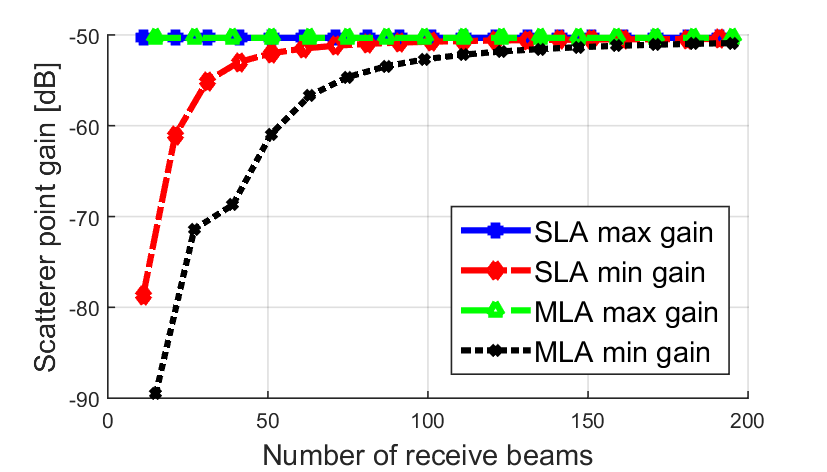
\includegraphics[width=\linewidth]{./images/results/4/gain_DAS.png}
        \caption{DAS}
    \end{subfigure}
    \quad
    \begin{subfigure}[t]{0.48\linewidth}
        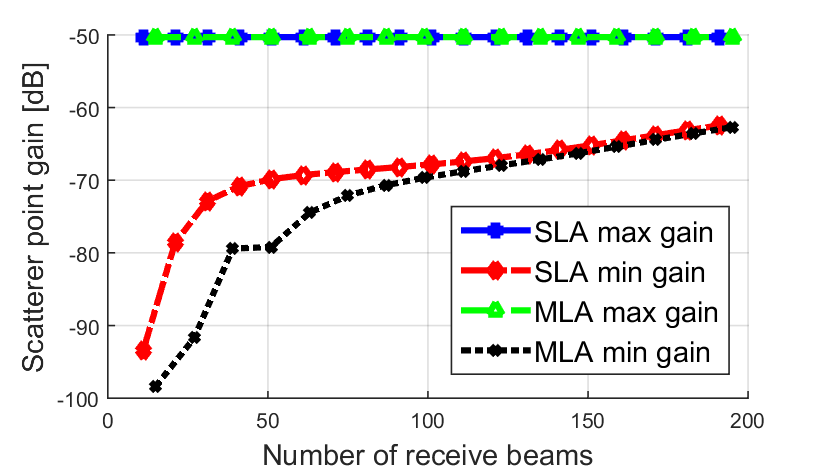
\includegraphics[width=\linewidth]{./images/results/4/gain_MV.png}
        \caption{MV}
    \end{subfigure}
    \quad
    \begin{subfigure}[t]{0.48\linewidth}
        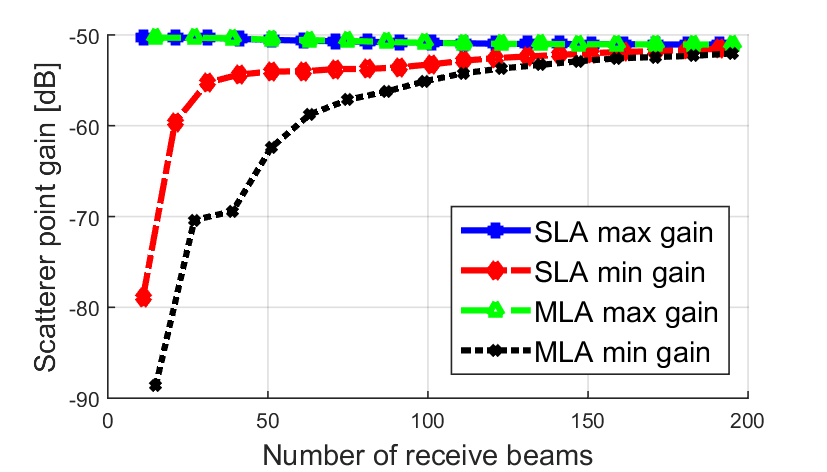
\includegraphics[width=\linewidth]{./images/results/4/gain_IAA-MBSB.png}
        \caption{IAA-MBSB}
    \end{subfigure}
    \quad
    \begin{subfigure}[t]{0.48\linewidth}
        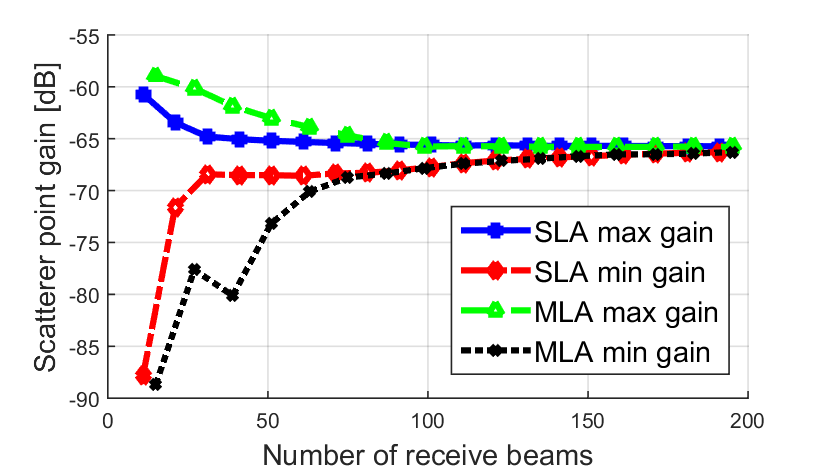
\includegraphics[width=\linewidth]{./images/results/4/gain_IAA-MBMB.png}
        \caption{IAA-MBMB}
    \end{subfigure}
	\caption{Maximum and minimum gains of single scatterer point at $40~$mm radius in a noiseless medium.}
	\label{fig:gain_comparison}
\end{figure}

With the issue of motion between frames explored with the naive MLA approach, we also want to analyze the effects of motion between beams and repeat the experiments of Section \ref{sec:twopoints_noiseless}.
Similarly as for Figure \ref{fig:two_points_static}, we simulate two points $s_1$ and $s_2$ at $40~$mm range such that both are on the trajectory of a transmit beam. With $d_B$ defined by Equation \ref{eq:dist_beams} as the distance between two beams, given a range $r$, $s_1$ and $s_2$ are laterally separated by $2 \cdot d_B = 0.75~$mm.
Figure \ref{fig:two_points_static_mla} shows the resulting beamformed images, as contour plots, with static scatterer points.
In that case, naive MLA seems to yield better results than perfect MLA (Figure \ref{fig:two_points_static}), with an apparent higher resolvability for all beamformers except DAS. The MV beamformer is even this time able to resolve the two points.
Since both points are on a transmit beam trajectory, the scalloping loss experienced in between them is not corrected for in the naive MLA approach, which, in this case, helps for resolving them.

\begin{figure}[ht]
    \centering
    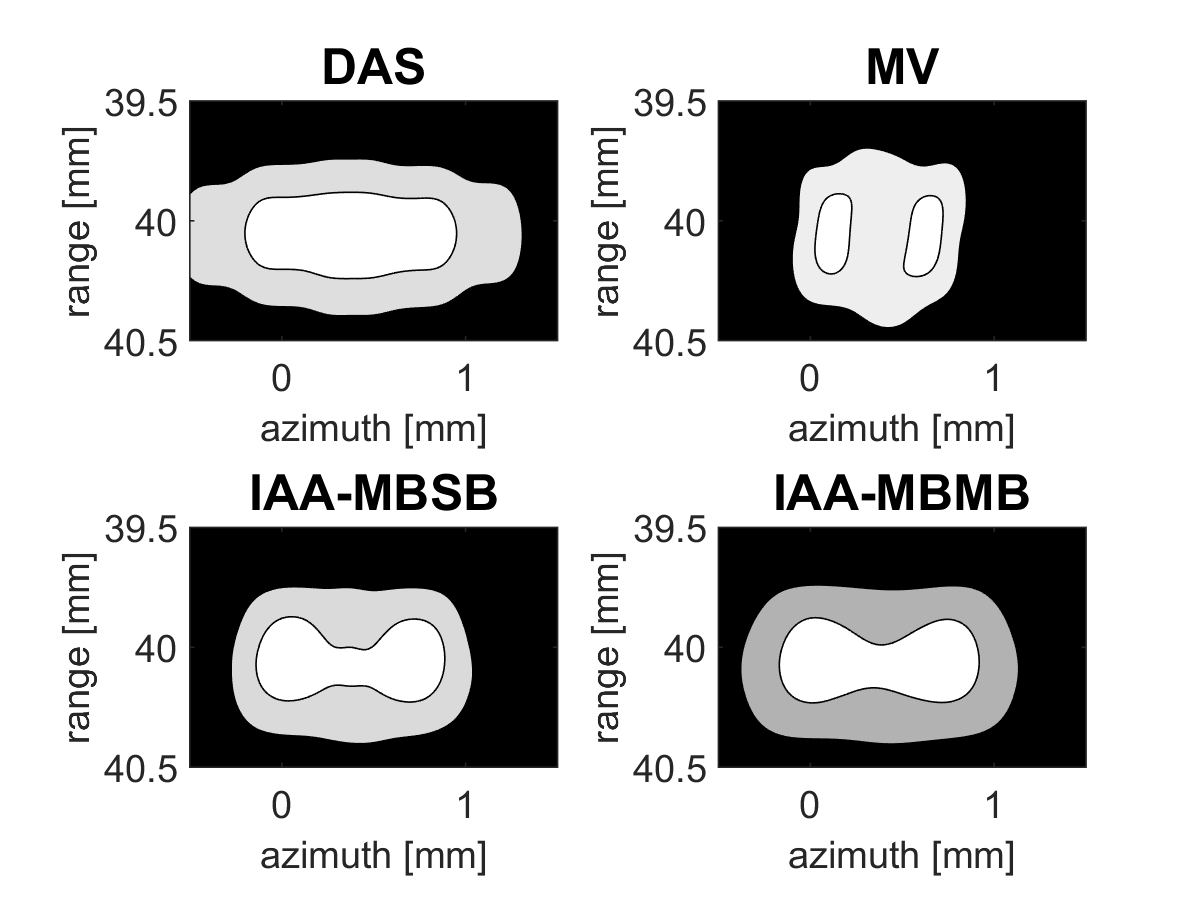
\includegraphics[width=\linewidth]{./images/results/4/two_points_static_mla.png}
	\caption[Contour plot of beamformed image, using naive MLA, with two closely-separated scatterer points in a noiseless medium]{Contour plot of beamformed image, using naive MLA, with two closely-separated scatterer points in a noiseless medium. Color levels are:  max-100, max-10 and max-3 dB.}
	\label{fig:two_points_static_mla}
\end{figure}

However, we can not always expect this lack of correction to be so advantageous for us.
Figure \ref{fig:two_points_linear_motion_mla} shows the results of the same scene as Figure \ref{fig:two_points_static_mla}, but with both scatterer points moving in various directions at $0.6~$m/s.
In this experiment, $s_1$ is still always guaranteed to hit the array's center transmit beam, but $s_2$ can experience scalloping loss.
Figures \ref{fig:mla_a}, \ref{fig:mla_e} and \ref{fig:mla_g} are good examples of $s_2$ experiencing visible scalloping loss, which is why it appears smaller than $s_1$ for the beamformed images from the MV and IAA-MBSB beamformers.

In Figures \ref{fig:mla_c}-\ref{fig:mla_h}, both scatterer points appear rippled for the DAS, MV and IAA-MBSB beamformers. This ripple is caused by the MLA approach that, in this case, creates three receive beams for each transmit beam.
The DAS beamformed image of Figure \ref{fig:mla_c} is a flagrant example as this ripple. We can see roughly three distinct range levels of the white shape (at $-3~$dB). Each range level represents a different transmit beam, at $0, 0.375$ and $0.75~$mm azimuth.

In every imaged scene, the IAA-MBMB yields impressive results compared to the other beamformers.
It manages to correct both for the visible scalloping loss and shape distortion induced by the naive MLA approach.
The IAA-MBMB beamformed images look identical to those of Figure \ref{fig:linear_motion_double} with perfect MLA.


\begin{figure}[ht]
    \centering
    \begin{subfigure}[t]{0.48\linewidth}
        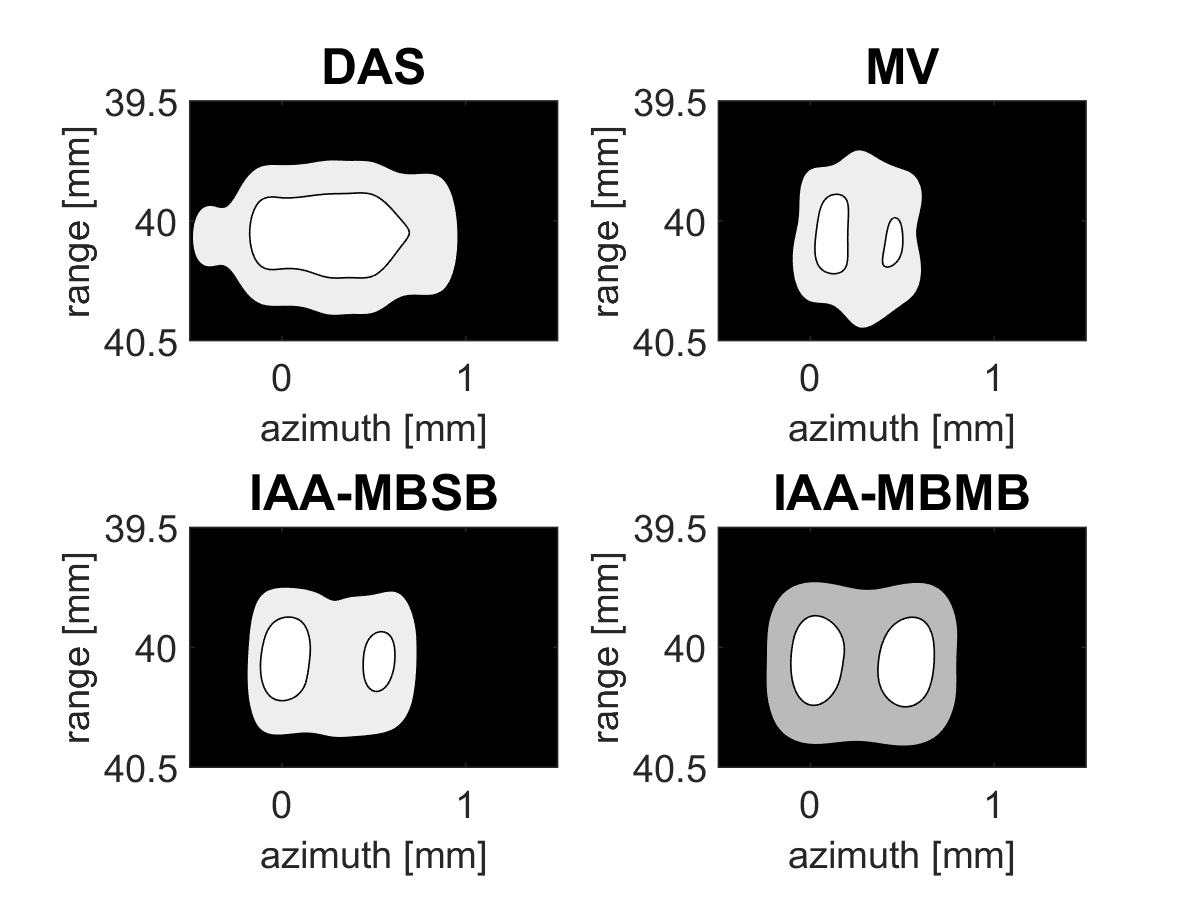
\includegraphics[width=\linewidth]{./images/results/4/motion_0_-06.png}
        \caption{$\boldsymbol{v}_s = (-0.6, 0)~m/s$.}
        \label{fig:mla_a}
    \end{subfigure}
    \quad
    \begin{subfigure}[t]{0.48\linewidth}
        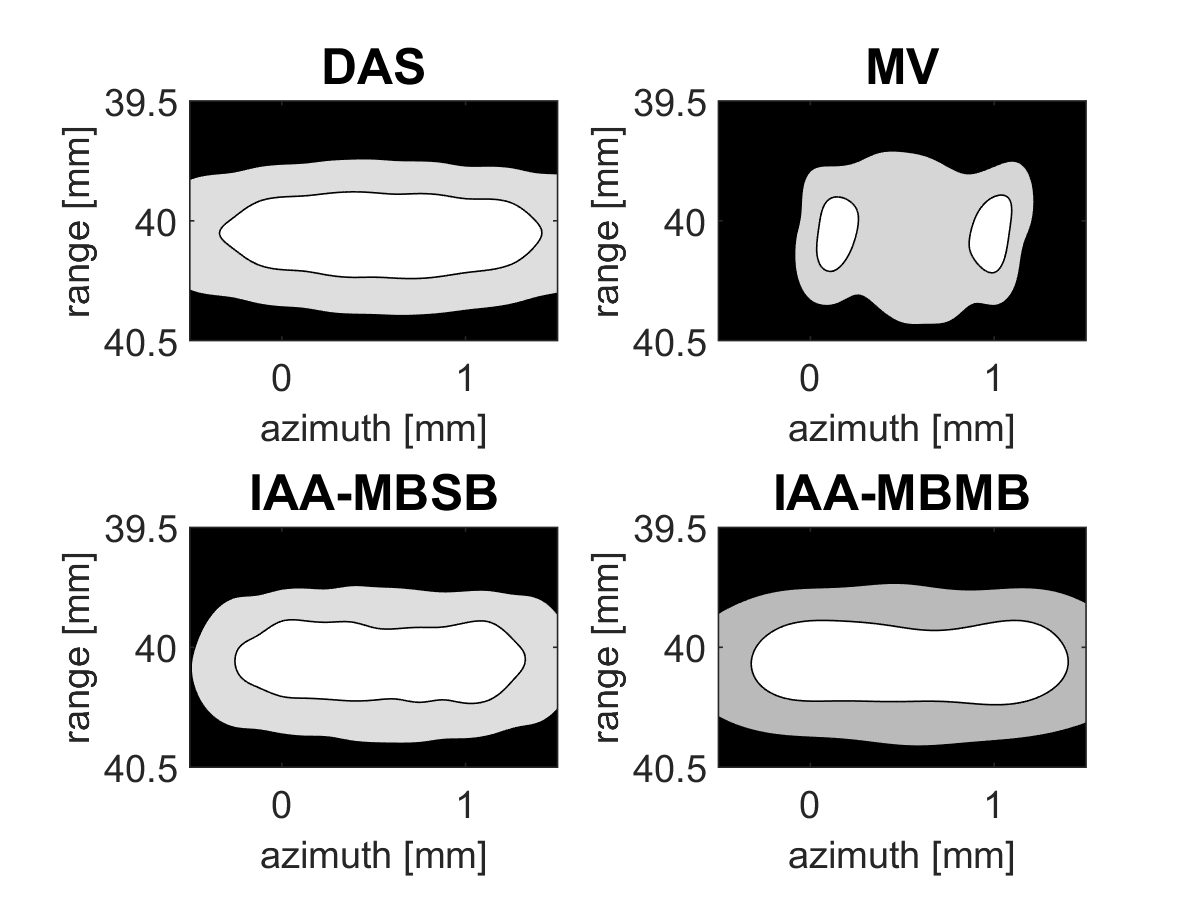
\includegraphics[width=\linewidth]{./images/results/4/motion_0_06.png}
        \caption{$\boldsymbol{v}_s = (0.6, 0)~m/s$.}
        \label{fig:mla_b}
    \end{subfigure}
    \quad
    \begin{subfigure}[t]{0.48\linewidth}
        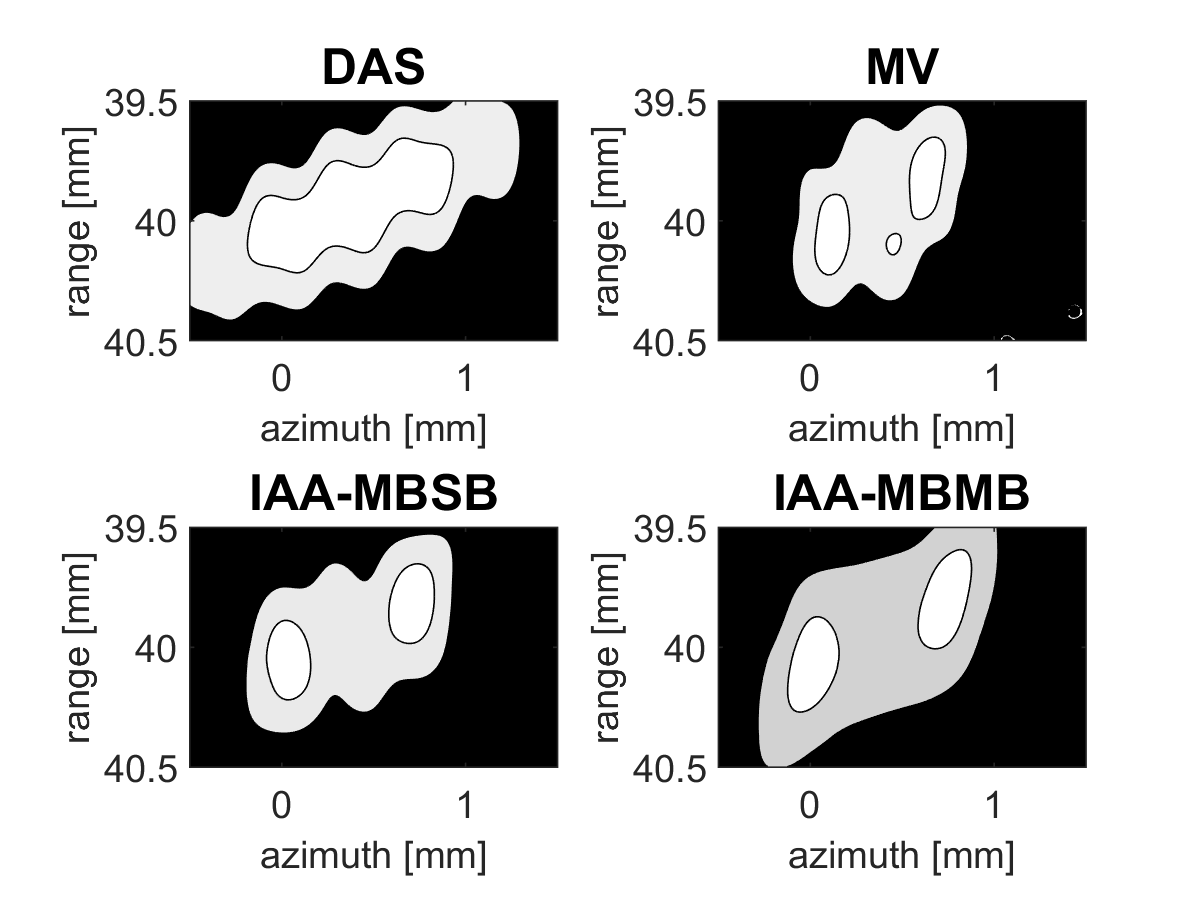
\includegraphics[width=\linewidth]{./images/results/4/motion_90_-06.png}
        \caption{$\boldsymbol{v}_s = (0, -0.6)~m/s$.}
        \label{fig:mla_c}
    \end{subfigure}
    \quad
    \begin{subfigure}[t]{0.48\linewidth}
        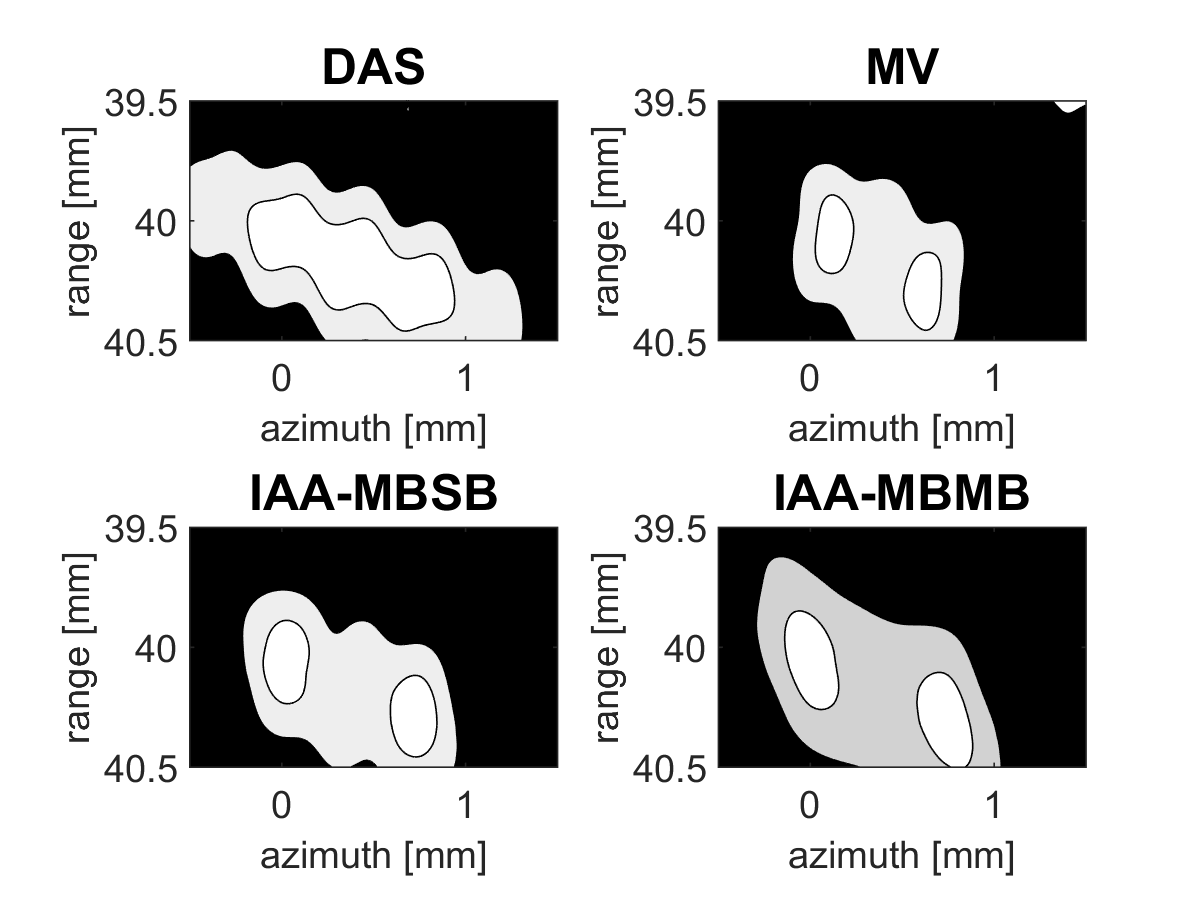
\includegraphics[width=\linewidth]{./images/results/4/motion_90_06.png}
        \caption{$\boldsymbol{v}_s = (0, 0.6)~m/s$.}
        \label{fig:mla_d}
    \end{subfigure}
    \quad
    \begin{subfigure}[t]{0.48\linewidth}
        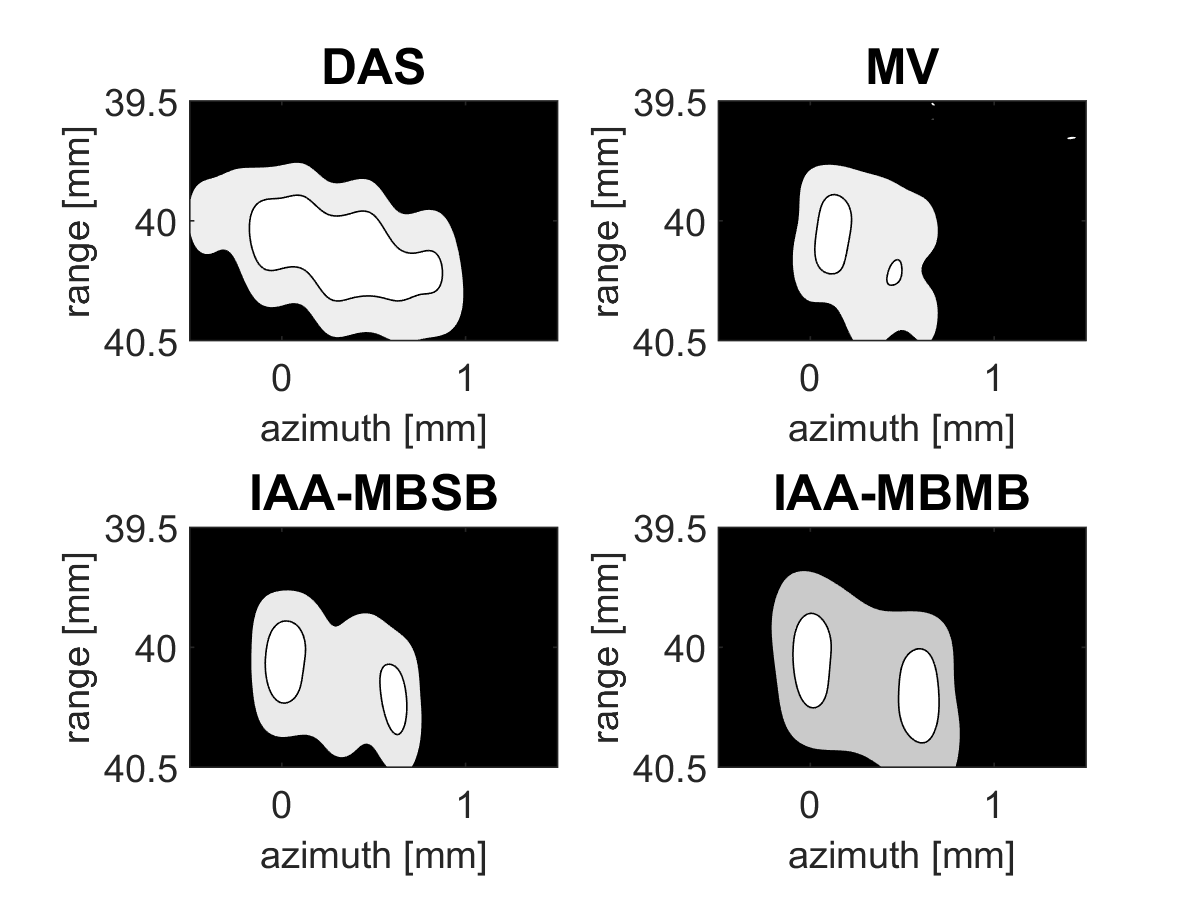
\includegraphics[width=\linewidth]{./images/results/4/motion_-45_-06.png}
        \caption{$\boldsymbol{v}_s = (-0.42, 0.42)~m/s$.}
        \label{fig:mla_e}
    \end{subfigure}
    \quad
    \begin{subfigure}[t]{0.48\linewidth}
        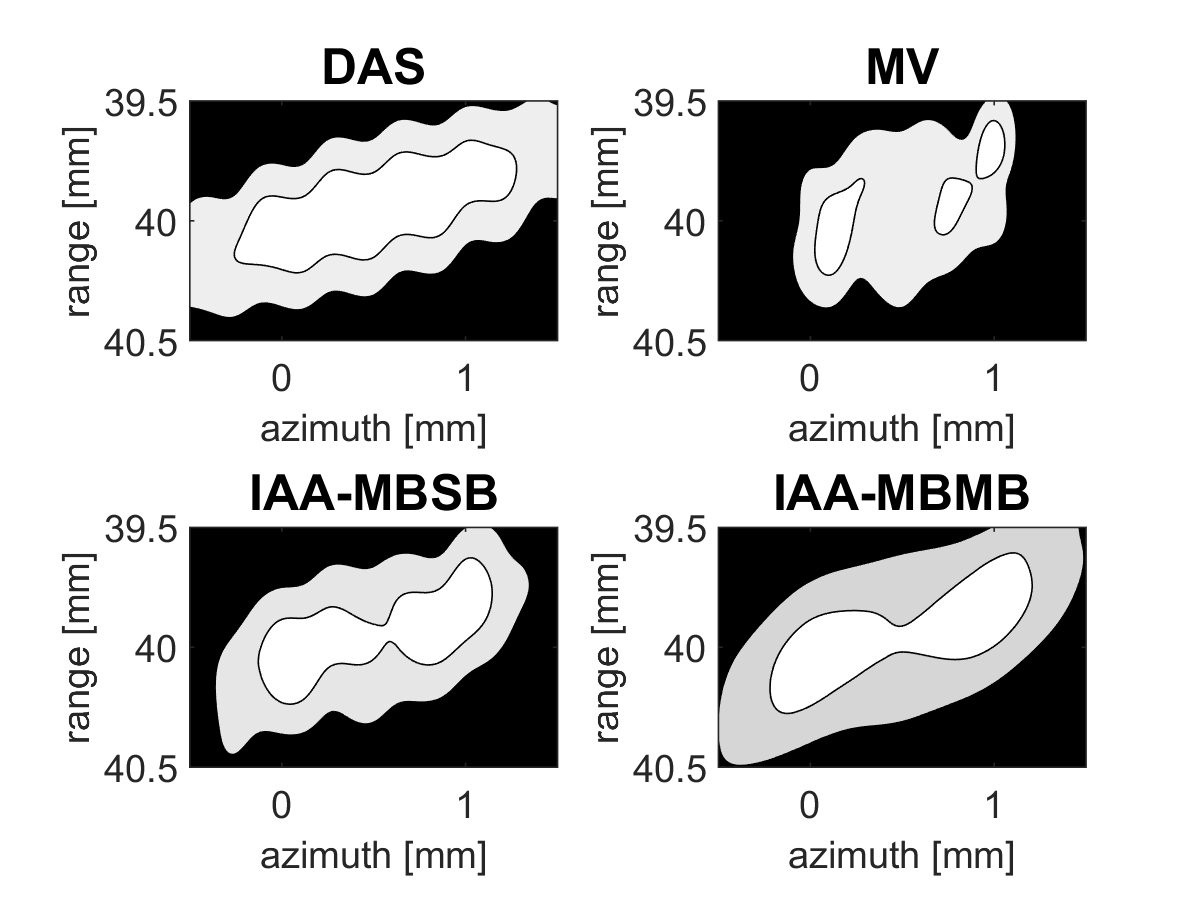
\includegraphics[width=\linewidth]{./images/results/4/motion_-45_06.png}
        \caption{$\boldsymbol{v}_s = (0.42, -0.42)~m/s$.}
        \label{fig:mla_f}
    \end{subfigure}
    \quad
    \begin{subfigure}[t]{0.48\linewidth}
        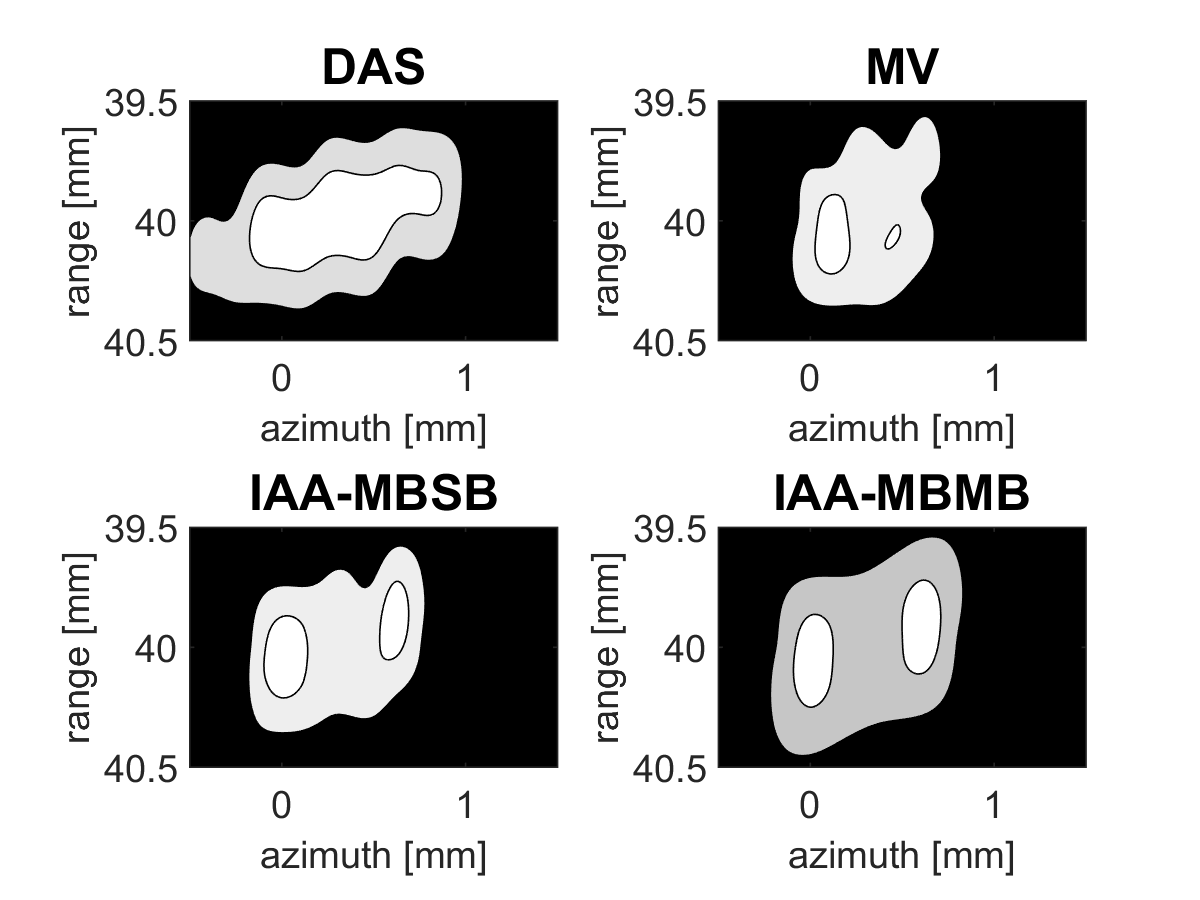
\includegraphics[width=\linewidth]{./images/results/4/motion_45_-06.png}
        \caption{$\boldsymbol{v}_s = (-0.42, -0.42)~m/s$.}
        \label{fig:mla_g}
    \end{subfigure}
    \quad
    \begin{subfigure}[t]{0.48\linewidth}
        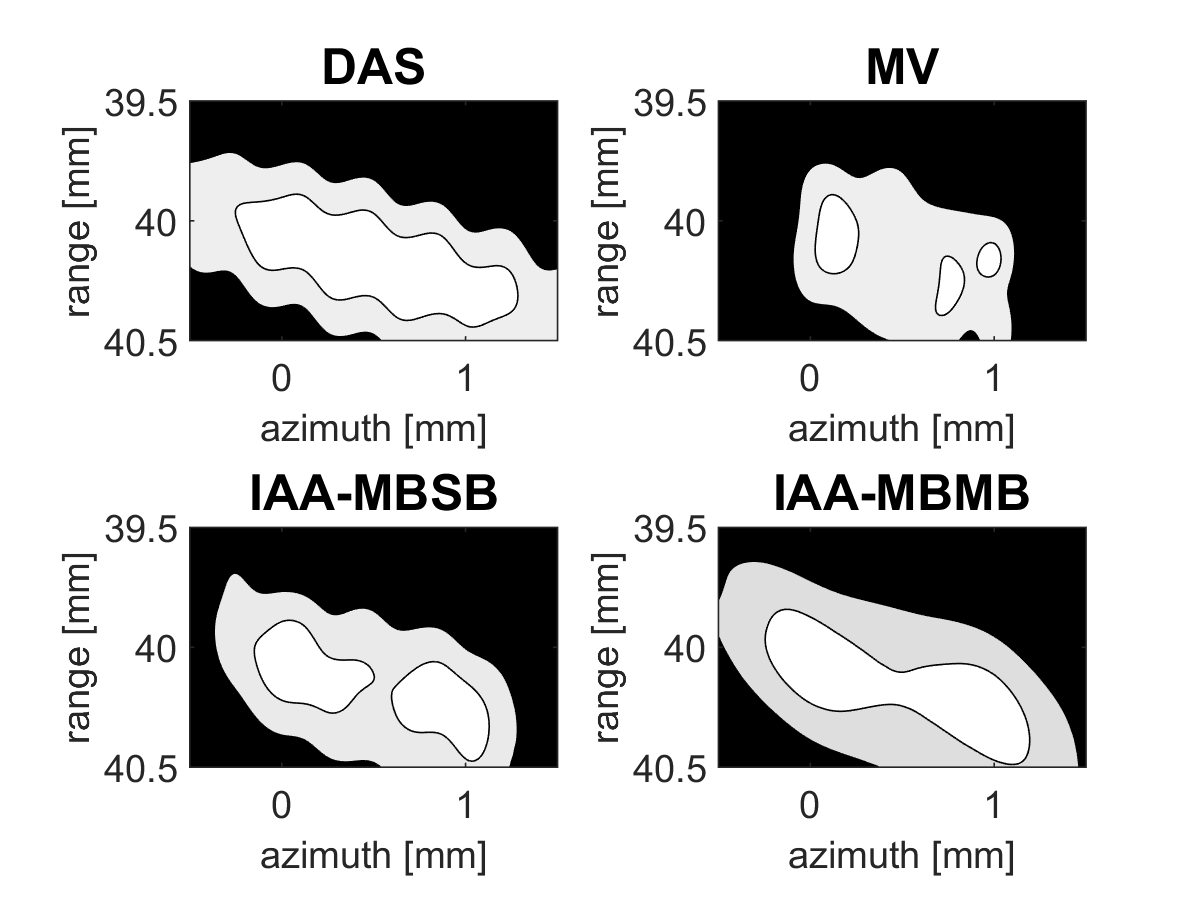
\includegraphics[width=\linewidth]{./images/results/4/motion_45_06.png}
        \caption{$\boldsymbol{v}_s = (0.42, 0.42)~m/s$.}
        \label{fig:mla_h}
    \end{subfigure}
	\caption[Two scatterer points, initially $0.75~$mm apart, in various linear motions $\boldsymbol{v}_s$ with $|\boldsymbol{v}_s|=0.6~m/s$ in a noiseless medium.]{Two scatterer points, initially $0.75~$mm apart, in various linear motions $\boldsymbol{v}_s$ with $|\boldsymbol{v}_s|=0.6~m/s$ in a noiseless medium. Contour plot levels: max-100, max-10 and max-3 dB.}
	\label{fig:two_points_linear_motion_mla}
\end{figure}